\section{Statistics and Probability}


\subsection{Problem 3.6}


\begin{figure}[!ht]
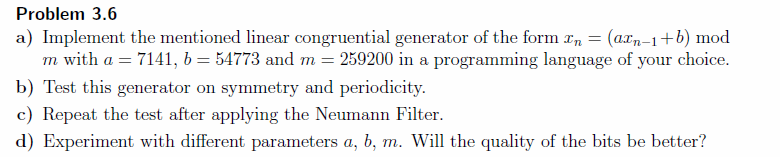
\includegraphics[width=1\textwidth]{chapters/images/desc-3-6}
\end{figure}


\subsubsection{a)}

\begin{lstlisting}[caption=Problem 3.6 a)]
class RNG:
	def __init__(self, pA = 7141, pB = 54773, pM = 259200):
		self.bits = [];
		self.x = 1;
		self.a = pA;
		self.b = pB;
		self.m = pM;
	
	def printParameters(self):
		print("a = " + str(self.a) + ", b = " + str(self.b) + ", m = " + str(self.m));
	
	def getRandomNumber(self):
		self.x = (self.a * self.x + self.b) % self.m;
		return self.x;
	
	def addNumbers(self, number):
		binNumber = bin(number)[2:];
		
		for bitNumber in binNumber:
			self.bits.append(int(bitNumber));
	
	def fillNumbers(self, iterations):
		for i in range(iterations):
			self.addNumbers(self.getRandomNumber());
\end{lstlisting}


\subsubsection{b)}

To test for symmetry and periodicity, new functions can be added to the RNG class from a).

\begin{lstlisting}[caption=Problem 3.6 b)]
	def makeSymmetryTest(self):
		sum = 0;
		
		for b in self.bits:
			sum += b;
		
		deviation = abs(0.5 - (sum / float(len(self.bits))));
		
		print("symmetry test:")
		print("deviation = " + str(deviation));
	
	def isPeriod(self, periodLength):
		nBits = len(self.bits);
		
		if periodLength * 2 > nBits: return False;
		
		iterations = int(math.floor(nBits / float(periodLength)));
		
		for i in range(periodLength):
			compareElement = self.bits[i];
		
			for j in range(1, iterations):
				key = j * periodLength + i;
				
				if key >= nBits: break;
				
				element = self.bits[key];
				
				if element != compareElement:
					return False;
		
		return True;
	
	def makePeriodicityTest(self):
		periodLength = -1;
		
		maximumPeriod = self.m * int(math.ceil(math.log(self.m, 2)));
		
		for i in range(1, maximumPeriod):
			if self.isPeriod(i):
				periodLength = i;
				break;
		
		print("periodicity test:");
		
		if periodLength < -0.5:
			print("no period found.");
		else:
			print("period length = " + str(periodLength));
\end{lstlisting}

Running these tests with the values $a = 7141$, $b = 54773$ and $m = 259200$ lead to the following results.

\begin{lstlisting}[caption=Result of 3.6 b), keywordstyle=\color{black}]
symmetry test:
deviation = 0.0266565772348

perodicity test:
no period found.
\end{lstlisting}

Note: The periodicty test had been aborted prematurely due to excessive run times of the program. With the large value $m$ and the conversion of the numbers into binary the length of the period cannot be calculated within reasonable time.


\subsubsection{c)}

Applying the Neumann Filter can also be realized as an additional function for the RNG class:

\begin{lstlisting}[caption=Problem 3.6 c)]
	def applyNeumannFilter(self):
		tempBits = self.bits;
		self.bits = [];
		
		nIterations = int(math.floor(len(tempBits) / 2.0));
		
		for i in range(nIterations):
			bit1 = tempBits[i * 2];
			bit2 = tempBits[i * 2 + 1];
			
			if (bit1 == 0 and bit2 == 1):
				self.bits.append(0);
			elif (bit1 == 1 and bit2 == 0):
				self.bits.append(1);
\end{lstlisting}

The results with the same values of b) after applying the Neumann Filter are:

\begin{lstlisting}[caption=Result of 3.6 c), keywordstyle=\color{black}]
symmetry test:
deviation = 0.000162239945826

perodicity test:
no period found.
\end{lstlisting}

Again, the periodicity test has been aborted prematurely.


\subsubsection{d)}

With the RNG class the values of $a$, $b$ and $m$ can easily be changed for further experiments:

\begin{lstlisting}[caption=Result of 3.6 d), keywordstyle=\color{black}]
a = 1, b = 1, m = 20
symmetry test:
deviation = 0.0769230769231

a = 20, b = 30, m = 100000
symmetry test:
deviation = 0.0624828117265

a = 214013, b = 2531011, m = 4294967296
symmetry test:
deviation = 0.0168803363686
\end{lstlisting}

Looking at the results the deviation tends to get smaller the higher the value of $m$ is. However, even with a value as little as 20 the deviation is somewhat reasonable.


\subsection{Problem 3.7}

\begin{figure}[!ht]
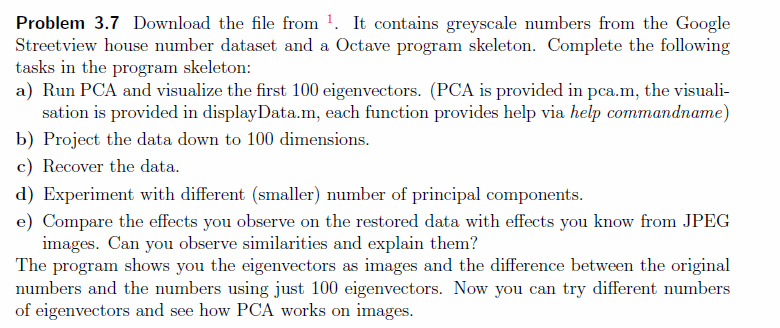
\includegraphics[width=1\textwidth]{chapters/images/desc-3-7}
\end{figure}

The first 100 numbers of the data looks like this:

\newpage

\begin{figure}[!ht]
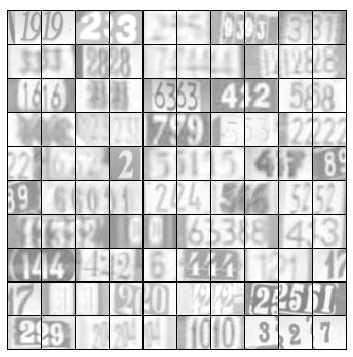
\includegraphics[width=1\textwidth]{chapters/images/figure-3-7-a}
\caption{The first 100 numbers of the data}
\end{figure}


\subsubsection{a)}

The top 100 eigenvectors can be dispayed the following way:

\begin{lstlisting}[caption=Problem 3.7 a)]
[U, S] = pca(X_norm);
eigenVectors = U(:,1:100);

displayData(eigenVectors');
\end{lstlisting}

The resulting visualization is:

\newpage

\begin{figure}[!ht]
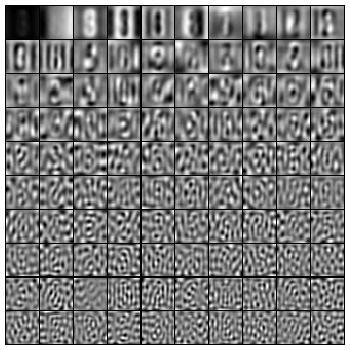
\includegraphics[width=1\textwidth]{chapters/images/figure-3-7-b}
\caption{The top 100 eigenvectors}
\end{figure}


\subsubsection{b)}

The data can be projected down to 100 dimensions in the following way:

\begin{lstlisting}[caption=Problem 3.7 b)]
Z = X_norm * eigenVectors;
\end{lstlisting}


\subsubsection{c)}

Recovering the data:

\begin{lstlisting}[caption=Problem 3.7 c)]
recoveredData = Z * eigenVectors';

displayData(X_norm(1:100,:));
displayData(recoveredData(1:100,:));
\end{lstlisting}

The recovered numbers look like this:

\begin{figure}[!ht]
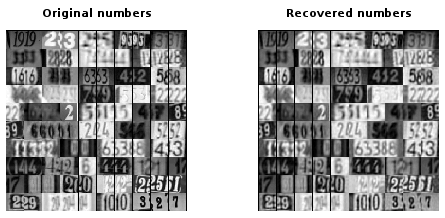
\includegraphics[width=1\textwidth]{chapters/images/figure-3-7-c}
\caption{The data using 100 principal components}
\end{figure}


\subsubsection{d)}

\begin{figure}[!ht]
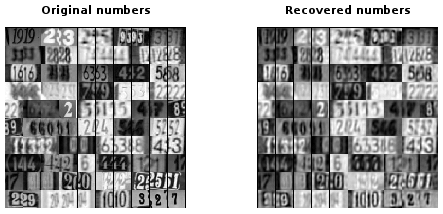
\includegraphics[width=1\textwidth]{chapters/images/figure-3-7-d1}
\caption{The data using 50 principal components}
\end{figure}

\newpage

\begin{figure}[!ht]
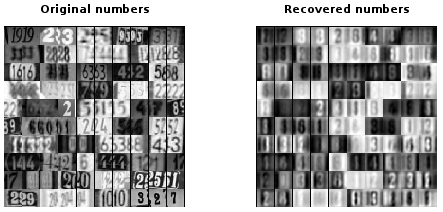
\includegraphics[width=1\textwidth]{chapters/images/figure-3-7-d2}
\caption{The data using 10 principal components}
\end{figure}


\subsubsection{e)}

By reducing the number of dimensions the detail gets lost in a similar way like the JPEG compression. This can be observed especially between two areas with a high color contrast.